\documentclass[a4paper]{article} 
\usepackage[utf8]{inputenc}
\usepackage{graphicx} 
\usepackage{subcaption}
\usepackage{stackengine}
\usepackage{listings} 
\usepackage{amsmath} 
\usepackage{color} 
\usepackage{hyperref} 
\usepackage[parfill]{parskip}
\usepackage{amssymb}
\usepackage[
    style=authoryear, 
    backend=biber, 
    maxcitenames=2, 
    mincitenames=1
]{biblatex}
\usepackage{etoolbox}
%\AtBeginEnvironment{quote}{\par\singlespacing\small}
\addbibresource{refs.bib}
\captionsetup[subfigure]{justification=raggedright, singlelinecheck=off, labelfont=bf}
\setstackgap{voffset}{5pt}
\setstackgap{hoffset}{5pt}

% Global setup for the main figure caption
% Global setup for the main figure caption
\captionsetup[figure]{
    font={sf,small},       
    labelfont=bf,            % Formats the caption as a block/box
    labelsep=period,       % Uses a hyphen (en-dash) as the separator: Figure 1 – Text
    justification=justified % Ensures the "box" look for full text blocks
}

% Setup for subfigures (titles above the images)
\captionsetup[subfigure]{
    font={sf,small},
    labelfont=bf,          % Bold (a), (b) if you use standard captions
    labelsep=period
}

% 2. Define a custom command for the floating labels
\newcommand{\floatlabel}[1]{\textsf{\textbf{\Large #1}}}

\title{Understanding Grammar Representation in the Human Brain via Information-Restricted LLMs} 
\author{Simone Esposito} 
\date{February 2026} 


\begin{document} 

\maketitle 

\section{Introduction}
\subsection{Importance of verbs and nouns in language}

Ever since the start of elementary school, identifying and distinguishing Grammatical Class (GC) – especially nouns and verbs – plays a fundamental role in the understanding of grammar. Researchers in the field of linguistic neuroscience have long examined whether this distinction was represented in the brain. However, this has proven to be particularly challenging, with many studies showing contradicting results. 

\subsection{Neuropsychological studies}

Early neuropsychological studies conducted experiments with aphasic patients who had strong impairments in the retrieval and production of nouns and verbs respectively. \textcite{damasio_nouns_1993}, for example, observed impairments in noun retrieval for two patients with damage to the \textit{left anterior and middle temporal lobe}, while the \textit{left premotor cortex} was named as a possible cause of the third patient’s impairment in the retrieval of verbs. This observation gave rise to the \textit{fronto-temporal} dichotomy, suggesting that nouns might be processed in temporal areas while verbs are processed in frontal areas.

However, subsequent studies have found contradicting results, with some patients showing frontal damage without verb deficits and temporal damage without noun deficits \parencite{damasio_neural_2001,de_renzi_sparing_1995}. Additionally, some of the verb deficits could be explained by the difference in imaginability of the words \parencite{crepaldi_clustering_2013}.

\subsection{Psycholinguistic Models}

\begin{itemize}
    \item \textbf{Lexicalist:} GC information is automatically retrieved upon retrieving the word.
    \item \textbf{Combinatorial:} GC is viewed as \textit{procedural knowledge.} Nouns/Verb category is treated as computational objects and only relevant for integration tasks.
    \item \textbf{Emergentist:} GC information is a property emerging from semantic constraints like nouns $\rightarrow$ objects and verbs $\rightarrow$ actions.
\end{itemize}

Another hypothesis for the apparent distinction is that the brain does not process GC \textit{per se} but rather the meaning that is usually associated with the word \parencite{vigliocco_nouns_2011}. Particularly, nouns are usually associated with \textbf{objects} while verbs tend to be associated with \textbf{actions.} This hypothesis also falls into the range of the \textbf{emergentist} views of psycholinguistics, wherein GC distinction is viewed as an emergent property driven by semantic constraints.
\section{Background} 

\subsection{Voxelwise Encoding Modelling} 

This thesis uses a method known as voxelwise encoding models, in which BOLD responses of each individual voxel are modelled as linear combinations of specific features. When the prediction accuracy for each voxel is then mapped onto the brain, areas that are better predicted may indicate that the corresponding part of the brain might encode information of the given features. The features themselves are generally nonlinear transformations of the stimuli onto a high-dimensional feature space.  

One prominent model \parencite{huth_natural_2016} constructs the features by computing, for each word in the stimulus, the co-occurrence between that word and 985 basic English words based on a large corpus of texts. This embeds each word in the stimulus onto a 985-dimensional vector, where similar words tend to correlate. This model has proven to be highly effective at predicting brain activity.  

\subsection{Contextual Embeddings} 
Nevertheless, the main shortcoming of that model is that the same word will always be mapped to the same embedding, regardless of context. For example, the word \textit{fine} in \textit{"I am fine," "I have to pay a fine,"} and \textit{"I used a fine brush"} all have completely different meanings, which might dilute the information in the features.  

To address this, language models (LM) started to be used to generate contextual embeddings. First, \textcite{jain_incorporating_2018} started by using Long Short-Term Memory networks (LSTM), then as technology improved, more advanced language models such as GPT-2 or Llama started to be used to generate such embeddings.  

To show that these contextual models actually relied on the context, the latter was scrambled and randomized, which, as expected, led to an overall worse performance. Nevertheless, there has not been a paper taking a closer look at what effect other kinds of context manipulation might have on prediction accuracy.

\section{Materials} 

\subsection{Stimuli} 

The speech stimuli consist of 11 short stories taken from \textbf{The Moth Radio Hour}, a storytelling program where true autobiographical stories are told in front of a live audience. These stimuli were used in previous papers (Huth et al., 2016), including the one where the response data was gathered (Deniz et al., 2019). These stories provide a naturalistic stimulus. 

Out of these 11 stories, 10 were used as training data while one 10-minute story was used as validation data. The latter was played two times during the experiment (in two separate scans) to which the responses were finally averaged across the two runs. 

These stories were then transcribed and stored as Praat's TextGrid objects, a text-based file format containing the transcription of the words spoken in the stories and the times when they were spoken. Additionally, the text grids also contained phoneme information which was not used in the project.  

\subsection{fMRI Responses} 

Each spoken (and written) story was presented during a separate fMRI scan. The length of each scan was the same as the story. The sampling rate was 2 seconds, so $1 \text{ TR} = 2 \text{ s}$. Each scan included 10 seconds (5 TR) of silence both before and after the story. These data were collected during 23-hour scan sessions that were performed on different days. MRI data were collected on a 3T Siemens TIM Trio scanner at the UC Berkeley Brain Imaging Center using a 32-channel Siemens volume coil.  

Each functional run was motion-corrected using the FMRIB Linear Image Registration Tool (FLIRT) from FSL 5.0 (Jenkinson and Smith, 2001; Jenkinson et al., 2002). All volumes in the run were then averaged over time to obtain a high-quality template volume. FLIRT was also used to automatically align the template volume for each run with the overall template, which was chosen to be the temporal average of the first functional run for each participant.  

The responses were provided as HDF files. For each subject and each modality, there were two files: one for the training stories and one for the validation story, for a total of 36 files. Each training file contains a dictionary with the stories as keys and the BOLD responses as values. Each validation file contains a dictionary with \textit{story\_11} as the key and the responses from both repetitions as values. 

The responses are represented as a 2D \lstinline{numpy} array with shape $(N_{TR} \times N_{voxels})$. The amount of TRs depends on the story, while the amount of voxels is unique to the subject. The response data also included the 10 seconds of silence before and after the story was played. 

\subsection{Features} 

To reproduce the original study, the 985-dimensional Eng1000 features were provided. 

To account for response variance caused by various modality-dependent nuisances, several additional features were provided. 

\subsubsection{Phonemes}  
A list of phoneme-time pairs was constructed for each of the 39 English phonemes. This list was then down-sampled to the fMRI acquisition rate. The result is a $(39 \times N_{TR})$ array. These features were used when fitting the model to the \textit{listening} responses.

\subsubsection{Letters} 
Similar to the phonemes, a 26-parameter model was created to represent the frequency of each of the 26 letters in the English alphabet that appeared in the written stories. This was also down-sampled to the sampling rate, resulting in a $(26 \times N_{TR})$ array. 

\subsubsection{Additional Features} 
To account for the highly variable speech rate both within and across stories, single-feature models were constructed. These count the number of words, number of phonemes, number of letters, and number of story speaker’s pauses that occurred during the acquisition of each fMRI volume (2.0045 s). To account for the variable word lengths during the visual presentation, a single-feature word length variation model was constructed by taking the variance of word lengths that occurred during the acquisition of each fMRI volume.

\subsubsection{Contextualized Embeddings}

The largest issue with the lexical \textit{english1000} embeddings is the lack of contextual information in the feature space. Put differently, the same word will be mapped to the same feature vector regardless of the context it is in. For example, the word \textit{fine} has a very different meaning in the sentences ``I am fine'' and ``I paid a fine.''

To account for this, I made use of \textit{contextualized embeddings} (CE), which as the name suggests, aim to include contextual information in the word embeddings. Such embeddings were introduced by the Long Short-Term Memory (LSTM) network ELMo \parencite{peters_deep_2018} and refined by the transformer model BERT \parencite{devlin_bert_2019}. 

High quality CEs can be generated using modern Language Models (LM). For my paper I decided to use GPT-2's embeddings, as it is commonly used in other related literature \parencite{schrimpf_neural_2021,tuckute_driving_2024}.

\textit{Tokenization}

Before a sentence or word can be embedded into vectors, it needs to be broken up into a set of token IDs $(t_1, \dots, t_n) \in V^n$ with $V$ being the vocabulary of all possible token IDs. Since single words can be broken up into multiple tokens, I need to keep track of which tokens are part of the context and which represent the target word. To do this, I first generate the tokens for the whole sentence $(t_1, \dots, t_n)$ to pass unto the LM, then just the tokens for the context $(t_1, \dots, t_m)$ to get the index $m < n$ where the target word starts. For this thesis, I used a context size of 20 words \parencite{pasquiou_information-restricted_2023}.

\textit{Initial Embeddings}

Upon passing on the tokens, GPT-2 first converts them into embedding vectors via a lookup table with a fixed embedding size $d_{emb}$, then adding those to their positional encoding vectors to generate the initial embeddings. These initial embeddings are non-contextual.

\textit{Hidden Layers}

The initial embeddings then go through a sequence of layers where they are first weighed using the attention mechanism \parencite{vaswani_attention_2023} then passed through a feed-forward network to enrich them with contextual information from surrounding embeddings, finally generating a new CE with the same size $d_{emb}$. Previous studies have found that the middle layers, e.g., Layer 8 for GPT-2 small, are best at predicting brain activity in VEMs \parencite{schrimpf_neural_2021,jain_incorporating_2018}.

\textit{Averaging}

The hidden state $H_8 \in \mathbb{R}^{n \times d_{emb}}$ contains the CE for the whole sentence. To get the vector of the target word, I first need to extract the embeddings of the target word's tokens $(h_8^{(m)}, \dots, h_8^{(n)})$. These embeddings are then averaged across tokens:
\[
    \overline{h}_8 = \frac{1}{n - m + 1} \sum_{i=m}^{n} h_8^{(i)}
\]

This yields the final CE for our target word.

\textit{Downsampling}

After repeating the process for each word $w_i \in (w_0, \dots, w_{N_{words}})$, I have an embedding matrix $E \in \mathbb{R}^{N_{words} \times d_{emb}}$. To be able to fit the features to the fMRI data, I need to downsample the CEs onto a feature space $F \in \mathbb{R}^{N_{TRs} \times d_{emb}}$ via a Lanczos filter \parencite{deniz_representation_2019}.

\subsubsection{Context Masking}

The masking of Parts of Speech (POS) was done automatically using Python's \texttt{spaCy} library. First, the target POS for the whole text is masked. This corresponds to applying the masking function $f_i: W_i \rightarrow W_i \cup \{'XXXX'\}$ to each story $S_i$, which replaces a word $w \in W_i$ with the redacting string if its POS corresponds to the target category, while leaving it unchanged otherwise:

\begin{quote}
    \textit{Original:} \dots So I was going up to \textbf{camp} and feeling pretty good about it and I decided on the \textbf{way} I would stop into Ithaca. I heard it was kind of a neat \textbf{town}. So I pulled off the \textbf{highway} into Ithaca and um it's on the southern \textbf{shore} of \textbf{lake} Cayuga\dots
    
    \textit{Masked (Nouns):} \dots So I was going up to \textbf{XXXX} and feeling pretty good about it and I decided on the \textbf{XXXX} I would stop into Ithaca. I heard it was kind of a neat \textbf{XXXX}. So I pulled off the \textbf{XXXX} into Ithaca and um it's on the southern \textbf{XXXX} of \textbf{XXXX} Cayuga\dots
\end{quote}

Afterwards, a sliding window of size $k=20$ moves over each word $w_{i,j} \in S_i$ to construct the context set:

\[ C_{i,j} = \{ f_i(w_{i,m}) \mid \max(0, j-k) \le m < j \} \]

where $w_{i,0} = \epsilon$ represents the empty context for the first word of each story.

\textit{Common nouns and Proper nouns}

\textit{Contractions}

\begin{figure}
    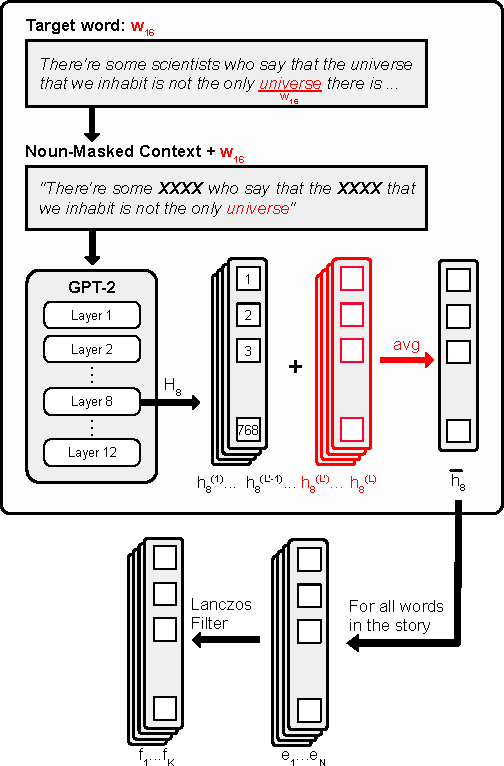
\includegraphics{figures/Fig1.pdf}
    \centering
    \caption{Example of the masked context embeddings generation. The max 20 words context is masked before going through GPT-2. 
    Extracting the hidden state $H_8$ at layer 8 yields the contextual embeddings for the context 
    and the target word. 
    The latter get averaged to produce the final contextual embedding for the target word. This process is repeated for each word in the story, 
    yielding a contextual $(N \times 768)$ embedding matrix. Finally, the embedding matrix is downsampled to match the fMRI sampling rate, 
    yielding the final $(K \times 768)$ feature space.
    The same procedure was applied to verbs, adjectives, adverbs, pronouns and interjections.}
\end{figure}
\section{Methods}  

\subsection{Contextual Embeddings Generation}

\subsection{Context Masking}
\subsection{Multiple Kernel Ridge Regression} 
\subsection{Permutation Testing} 
\subsection{FDR Correction} 

\subsection{Visualization} 
\label{sec:vis} 
\newpage
\section{Results} 
\begin{figure}
    \begin{subfigure}{\textwidth}
        \centering
        \stackinset{l}{5pt}{t}{5pt}{\floatlabel{a}}{
            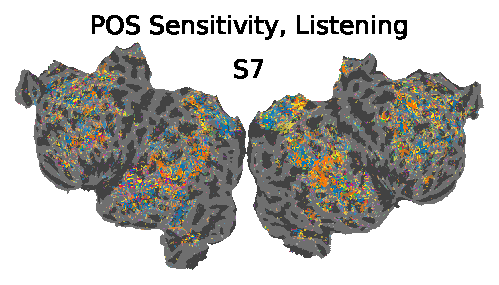
\includegraphics{figures/subject07-listening-all.pdf}
        }
    \end{subfigure}
    \begin{subfigure}{\textwidth}
        \centering
        \stackinset{l}{5pt}{t}{5pt}{\floatlabel{b}}{
            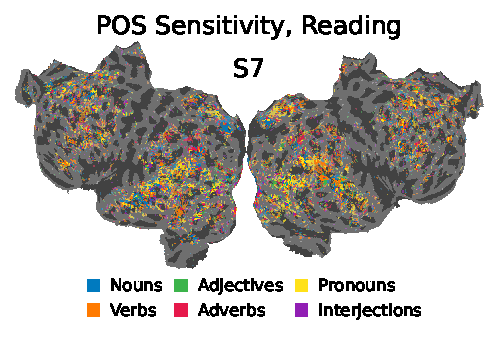
\includegraphics{figures/subject07-reading-all.pdf}
        }
        \end{subfigure}
    \begin{subfigure}{\textwidth}
        \centering
        \stackinset{l}{5pt}{t}{5pt}{\floatlabel{c}}{
            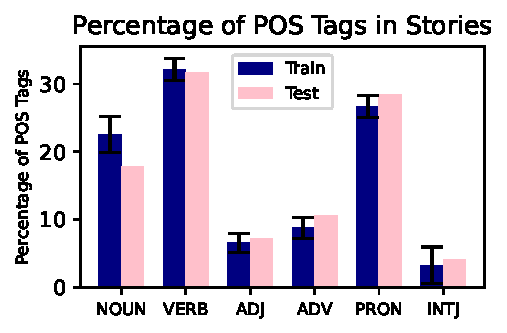
\includegraphics{figures/pos_distribution.pdf}
        }
    \end{subfigure}

    \centering
    \caption{Part of Speech sensitivity across the brain using all POS: nouns, verbs, adjectives, adverbs, pronouns and interjections.
    \textbf{a} Voxelwise model r values in the listening modality using POS-masked contextual embeddings were subtracted from the r values of the baseline contextual model to 
    get the drop in accuracy. The drop in accuracy for each POS was then ranked for each voxel individually and the greatest drop was plotted on the flatmap in the respective color
    \textbf{b} Voxels are colored using the same procedure as in \textbf{a} but for the reading modality. 
    \textbf{c} Distribution of POS tags in the training stories and the validation story. 
    The percentage of each POS tag was calculated by counting the number of words with that tag and dividing it by the total number of words in the story. 
    The average percentage across the 10 training stories is plotted on the left, while the percentage for the validation story is plotted on the right.}
\end{figure}
\newpage
\section{Discussion} 
\newpage
\section{Literature}
\printbibliography
\end{document}